\documentclass[12pt, notitlepage]{article}
\usepackage[bottom = 5cm, top = 5cm, left = 3cm, right = 3cm]{geometry}
\usepackage[english]{babel}
\usepackage[utf8]{inputenc}
\usepackage[table]{xcolor}
\usepackage{graphicx, booktabs, tikz, csquotes, subfig, enumitem, dcolumn, pdfpages}
\usepackage[font=normalsize]{caption}%,labelfont=bf
\usepackage{subcaption}

\renewcommand*\rmdefault{ppl}

\usepackage{setspace}
\setstretch{1.5}

\usepackage[]{titlesec}
    \titleformat*{\section}{\large\bf}
    \titleformat*{\subsection}{\normalsize\it}

% Bibliography
% \usepackage[natbibapa]{apacite}
\usepackage[round]{natbib}
% \renewcommand{\bibliographytypesize}{\normalsize}
\setlength{\bibsep}{5pt}

\usepackage[colorlinks = TRUE, allcolors = blue]{hyperref}

\widowpenalty=10000
\clubpenalty=10000

\title{\Large Do TJ policies cause backlash?\\Evidence from street name changes in Spain}
\author{Francisco Villamil\thanks{Juan March Institute--Carlos III University of Madrid} \and Laia Balcells\thanks{Georgetown University}}
\date{\today\\\vspace{5pt}Word count:}

\begin{document}

\maketitle

\begin{abstract}
\setstretch{1}
Memories of old conflicts often continue to be present in national politics long after these conflicts end. The debates about the Confederacy in the United States, the Nazi period in Germany, or the Francoist regime in Spain suggest that these are sensitive topics that might increase political polarization, particularly when transitional justice policies are implemented to address grievances. One such policy recently debated in the US and Spain is the removal of public symbols linked to past authoritarian regimes. However, the empirical evidence on their impact is still limited. This article attempts to fill this gap by exploring the impact of removing Francoist street names in Spain. We analyze whether recent name changes have increased electoral support to the new far-right party Vox. Using cross-sectional and difference-in-differences analyses, we show that removing Francoist street names has led to a shift to far-right preferences. Results suggest that revisiting the past and trying to redress the victims' grievances might cause a backlash among those ideologically aligned with the perpetrator.

\vspace{5pt}
\noindent
\textbf{Keywords:} transitional justice, voting, conflict memories, Spain

\end{abstract}
\setstretch{1.5}


\newpage
\section*{Introduction}

Memories of contested historical events continue to shape domestic politics across the world.
In the United States, the Black Lives Matter movement has sparked a debate over Confederate symbols and the public display of a contentious past related to the Civil War and slavery.
The removal of these symbols, as transitional justice (TJ) measure, is defended on the grounds that they represent ideas that are no longer acceptable, impeding reconciliation.

Yet, their removal is not free of controversy.
% Indeed, the debate over the Confederate symbols became more salient after the 2015 mass shooting at a historic African-American church in South Carolina, where the killer had been found to be inspired by the heritage of the Confederacy \citep[e.g.][]{Palmer:2018aa}.
% Yet the removal of public symbols is not free of controversy.
In the South of the United States, there have been several instances of right-wing or white supremacist protests when statues of Confederates have been torn down.
In some cases, these protests have turned violent.
% Recent instances of political violence in the US have been directly related to the memories of the Civil War and the Confederacy.
The 2017 `Unite the Right rally' in Charlottesville, Virginia, opposing the removal of a Robert E Lee statue, quickly escalated into violence and resulted in the death of one person when a white supremacist drove his car into a crowd of counter-protesters.

Does this type of TJ policy cause backlash in the form of a shift to radical, right-wing positions?
% This phenomenon is not unique to the US.
% In Germany, Alternative for Germany (AfD) has recently drawn criticism because of their revisionist view of the national past.
% The AfD co-leader claimed in 2018 that the Nazi era was just a small episode in German history, while another AfD leader said that the Berlin Holocaust Museum was a ``monument of shame'' \citep{Laub:2018aa}.
% In Poland, there is a heated debate about the role of the country during World War II, which has contributed to increased political polarization.
% In 2018, the right-wing Law and Justice party changed the National Memory Law, ``threatening to prosecute anyone claiming that the Polish Nation was responsible for Nazi crimes'' \citep[][183]{Zubrzycki:2020aa}.
This question is the focus of this article.
In particular, we explore a potential backlash effect of the removal of public symbols linked to the Francoist regime in Spain.



We focus on Spain, where memories of the Civil War, a conflict that ended over 80 years ago, are still a source of fierce political debates and are likely behind recent dynamics of ideological polarization.
In particular, one of the main pillars in the discourse of the up and coming far-right party, Vox, is challenging what they refer to as the `manipulation of history' by the Left.
This manipulation is, according to this view, engraved in the Law of Historical Memory passed by a Socialist government in 2007, aimed at redressing long-held grievances and promoting reconciliation.
While this Law had a broad support in Spanish society, a significant proportion of the population---mostly at the right of the political spectrum and/or victimized by the leftist armed forces during the Spanish civil war (1936-1939)---disagreed with some of its policies \cite{Aguilar:2011aa}.%\footnote{For example, in the CIS 2760 poll data, around 20 percent of the respondents disagreed with the statement ``There should be a monument to all the victims of Francoism", and over 20 percent of the respondents disagreed with removing Francoist symbols from public spaces.}

%Previous works

In this article, we focus on the impact of the changes brought about in Spain by the 2007 Law of Historical Memory.
Among other things, this new law included a mandate to remove Francoist symbols from public spaces, including street names related to the Francoist regime.
Even though many local governments had already changed Francoist street names since the transition to democracy in the late 1970s, the passage of the 2007 Law of Historical Memory included a legal mandate to remove the remaining Francoist symbols.
%This law backed local associations that pressured local governments to remove the symbols still in place, either because of inertia or ideological intention.

We study whether the removal of Francoist street names generated a preference shift towards far-right positions among a subset of the population.
In particular, we look at the emergence and rise of Vox, a new far-right party.
Originated from a split within Partido Popular, the mainstream center-right party, Vox represents a hard version of Spanish nationalism. Its discourse glorifies Spain's imperial past and its national unity. It also condemns peripheral nationalisms and any attempt at redressing the official memory imposed by the Franco regime.
Mainly fuelled by the Catalan conflict and the rise to power of a left-wing government after a motion of no confidence in June 2018, the party became increasingly popular in late 2018.
Its electoral support increased from a mere 0.2\% of the vote in the 2016 elections to more than 10\% in the April 2019 elections and over 15\% in the November 2019 elections.
In this study, we exploit variation in support for Vox as a latent measure of authoritarian and far-right preferences, and probe whether the removal of Francoist street names accounts for this variation.
Additionally, we also explore whether the effects of the name removals are linked to an increase in local political polarization or a general shift to the right.

% Results support evidence for the authoritarian backlash hypothesis, in other words, that the removal of Francoist public symbols produced an authoritarian backlash, radicalizing right-leaning individuals and increasing political polarization.
Our results support evidence for the authoritarian backlash hypothesis.
The cross-sectional analyses show there is a correlation between the removal of Francoist streets (any time in the last two decades) and electoral support for Vox in 2019 elections.
In order to get closer to a causal identification, we develop a difference-in-difference (DiD) design where we explore the impact of Francoist street name removals on the growth of Vox electoral support between June 2016 and April 2019 elections.
Comparing only municipalities that still had Francoist street names in June 2016, we show that Vox support increased around 6\% more in municipalities where there was a removal of Francoist street names between June 2016 and April 2019. Interestingly, we find that support for the center-right party (PP) decreased a 8\% in those same municipalities, but that support for the the main center-left party (PSOE) did not vary.
The fact that Vox increased its electoral support at the expense of a more moderate right-wing party (PP) suggests that TJ politics is increasing local polarization, rather than bringing a general shift to the right.

The politics of memory and the revision of a country's history are key issues in contemporary politics.
National traditions and symbols across the world are being criticized because of their racial or ideological overtones.
Even though those who support these revision policies usually claim that they promote reconciliation, our argument is that can also have the unintended side effect of increasing political polarization.

%Our findings stand in contrast with previous works that find a reconciliatory effect of related measures, such as transitional justice museums \citep{Balcells:2020aa}.
%However, we argue that this difference might be due to the distinct nature of each measure and the degree to which key political actors are able to interpret or weaponize different policies to their own interest.
%In order to achieve reconciliation and the redress of grievances, policy makers need to plan ahead the design of transitional justice or revisionist policies, and they should keep in mind the capacity of political actors to manipulate them.

\section*{The consequences of TJ policies}

After regime transitions or violent episodes, states often confront the need to come to terms with the past.
To this end, states rely on different TJ policies, including legal responses such as trials and amnesties or setting up truth commission, museums, or memorials \citep{De-Brito:2001aa, Elster:2004aa, Balasco:2013aa}.
The politics of memory, which involve ``the shaping of collective memory by political actors and institutions'' \citep[][176]{Zubrzycki:2020aa}, are a crucial component of these policies.
All these measures aim to serve justice, redress grievances, and avoid the relapse of conflicts.
However, the short-term and long-term and consequences of TJ are not clear.

Several scholars have long praised TJ policies as a necessary part of reconciliation in postconflict situations or after regime changes.
The argument usually states that these policies increase the prospect for democracy \citep{Kritz:1995aa, Elster:2004aa, Sikkink:2007aa} and reduce the risk of future conflict by increasing accountability for repressive acts committed by the state \citep{Kim:2010aa, Meernik:2010aa}.
TJ policies promote reconciliation because they redress individual grievances and, particularly in ethnic conflicts, help dismantle the idea that the opposite group is collectively responsible for the crimes \citep{Scharf:1997aa, Akhavan:1998aa, Hayner:2001aa}.

Other authors argue that the positive view on TJ policies is overly optimistic, and that there is little evidence in support of a beneficial effect of TJ\citep{Mendeloff:2004aa, Thoms:2010aa, Daly:2011aa}.
Some works even claim that TJ policies can have a negative effect on reconciliation and conflict, because the exclusive reliance on prosecution and accountability can bring about social tensions in divided societies \citep{Goldsmith:2003aa, Snyder:2004aa}.
The idea that TJ policies can hinder reconciliation because they might intensify old hatreds and divisions was precisely one of the arguments held by conservative sectors in Spain against the 2007 Law of Historical Memory. Indeed, the debates about the past related to these TJ policies seem to have played a meaningful role in building a successful electoral discourse among populist right-wing parties in some European countries \citep{Martin:2020aa}.

We explore the effects of a particular subset of TJ policies, symbolic policies, and we use data from Spain to analyse their impact on political behavior.

%Previous research has paid close attention to the formal justice mechanisms of TJ policies, and particularly their effects on the recurrence of conflicts.
%However, part of the disagreement might stem from the fact that TJ include a wide array of different policies and mechanisms, each of which might have different effects.
%Some works find evidence of this idea, and suggest that the overall effect of TJ policies is contingent on the balance between different measures \citep{Olsen:2010aa, Loyle:2017aa}.
%Yet, we know much less about the specific effects of less formal measures of TJ and, particularly, about their effects on public opinion.
%Even if the overall goal of TJ policies is to avoid the relapse of conflict and increase the prospects for reconciliation, many of the mechanisms through which they are claimed to work are grounded on their attitudinal impact.

%Two recent works constitute a partial exception to this gap.
%\cite{Capoccia:2020aa} study the effects of TJ trials on prodemocratic attitudes in West Germany, and find that the effect %depends on the type of punishment and on the ethnic identity of the defendants.
%Using experimental evidence on the effect of visiting a TJ museum in Chile, \cite{Balcells:2020aa} find that some politics of memory might have a positive effect on reconciliation.

%All in all, our knowledge on the attitudinal effects of different TJ policies is limited.
%The need for more evidence on this is particularly important if we consider that the general effects of TJ policies are not homogenous.
%We try to contribute in filling this gap using empirical evidence from Spain, focusing on the changes brought about by the 2007 Law of Historical Memory.
%Specifically, we probe into the local effect of the removal of public symbols on political preferences.

\section*{Conflict memories and authoritarian backlash in Spain}

In order to explore the effects of the politics of memory, we exploit two recent phenomena in Spanish politics: the consequences of the Law of Historical Memory and the recent rise of a far-right party, Vox, whose discourse rests heavily on the version of Spanish nationalism supported by Francoism.

First, the Law of Historical Memory, promoted by a left-wing government and passed by the Congress of Deputies in 2007, was an attempt to redress long-held grievances by the victims---and their relatives---of the Civil War and the Francoist regime.
Among other things, it formally condemned the Francoist regime and included provisions for the removal of Francoist symbols from public spaces, such as street names and monuments.

Many local governments had already changed Francoist street names in the years since the transition to democracy.
For instance, the \textit{Paseo de la Castellana} and the \textit{Avinguda Diagonal}, two of the main arteries of Madrid and Barcelona, respectively, were named \textit{Avenida del Generalísimo Franco} until 1979.
However, these changes depended on an active decision made at the local level.
In many places, either because the wartime cleavage was not relevant enough or because local politicians actively rejected the change, many streets were still named after Francoist symbols or key figures.
The 2007 Law prompted local governments to act and offered local associations a legal platform to pressure their local councils to promote street name changes.
%\footenote{In fact, the Law of Historical Memory promoted and funded local `memory associations' that reviewed the local history and organized the exhumation of local mass graves.}

These policies were hotly contested by particular sectors of Spanish society. Even from the very first years of democratic rule, rightist parties rejected the change of street names or the removal of public monuments by saying that `stirring history' only brought old-seated divisions back \citep[e.g.][]{Fuente:1980aa}.\footnote{The exhumation of Francisco Franco from the Valley of the Fallen in late 2019 is probably the latest high-key example of the implementation of this law and the political tension it brought about \citep{Taladrid:2019aa}.}

Second, we focus on electoral support for Vox as a proxy of a backlash to ideological positions closer to the Francoist regime.
Vox is a relatively new far-right party in Spain which promotes a discourse based on authoritarian conservatism and a hard-line version of Spanish nationalism. It shares with other populist right-wing parties in Europe a nativist ideology and a rejection of immigration, gender policies, and the social welfare state \citep{Turnbull-Dugarte:2019aa, Turnbull-Dugarte:2020aa}.
%Even though it was formed in 2014, Vox remained relatively unknown until 2018, when it became increasingly popular, mainly because of the Catalan conflict and the rise to power of a left-wing government.
%While in 2016 elections it got 0.2\% of the total votes and no seats in parliament, this number increased to more than 10\% and 15\% in April 2019 and November 2019 elections, respectively.

The most relevant aspect of its discourse for this study is the use they made of the issue of historical memory in Spain.
Characterizing the Law of Historical Memory as an instrument of leftist propaganda, Vox campaigned on the national unity of Spain as a way of leaving behind historical divisions and enacted the figure of Francisco Franco as an important political leader who brought peace and stability to the country.
Interestingly, this discourse directly inherits the `forgetting' policy developed by the Francoist regime in the postwar period, which reinterpreted the  Second Republic as a period of chaos and instability and the military rebellion of 1936 as a crusade to reestablish order \citep{Palomares:2004aa}.

We make use of these two events to assess whether the politics of memory in Spain caused a backlash towards positions closer to the ideology of the Francoist regime.
Assuming that electoral support for Vox is related to authoritarian ideology and a more benign view of the Francoist regime, we measure whether the removal of Francoist street names is related to a local increase in support for Vox.
Our expectation is that the relationship will be positive, supporting the backlash hypothesis.

\section*{Empirics}

Our unit of analysis is the municipality, and we develop two groups of analyses.
First, we use a cross-section of all municipalities and test whether the removal of Francoist streets since 2001 is correlated with higher support for Vox in both 2019 elections.
Second, in order to get closer to a causal identification, we develop a difference-in-differences analysis on the increase in electoral support for Vox between June 2016 and April 2019 elections, using the removal of Francoist street names as our main independent variable and limiting the sample only to those municipalities that still had Francoist street names in June 2016.

\subsection*{Francoist street name removal}

To build our main independent variable, we downloaded data identifying all the streets in Spain at different points in time from the Census Street Map of the National Statistical Institute or \citet{INE:2020aa}.
In particular, the INE offers data for every six-month period since January 2011,\footnote{Specifically, it offers the official data for June 30th and December 31st.} plus a snapshot of the streets and their names existing in July 2001.
Using the official ID number for each street, which remains constant, we are able to track the change in street names over time.

Using this setup, we identified streets named after Francoist symbols or figures.
We used as a starting point the list published by the Madrid City Council in 2017, where they proposed a list of 52 street names to be removed, following a report by a specially designated commission\footnote{The full list and the reasons for the choice of each street name is available online at https://bit.ly/37cLGgk (accessed 26/11/2020).}.
We expanded the list manually selecting from the most commonly changed street names in the data.
Indeed, among all the changes between 2001 and 2020, the five most commonly removed street names were all key Francoist figures: `Jose Antonio', `Calvo Sotelo', `General Mola', `Generalísimo', and `General Franco'.
We include in the Appendix the full list of Francoist street names.

Figure~\ref{fig:changes_time} shows the number of changes during every six-month period between January 2011 and July 2020.
Figure~\ref{fig:fs_year} shows yearly data on the share of all the streets that had Francoist names.
The descriptives show that there was an increase in Francoist name removal after 2016, precisely the period we use in our difference-in-differences analyses.
These relatively late changes were probably due to the time it took for the 2007 Law to be implemented at the local level.
The decrease in votes for the mainstream right-wing party in the 2015 local elections, the fact that the initiative to change street names was local, and the time any legal battle or pressure campaing would take probably explain this lag.
However, this increase could introduce a bias in the results if it was related to political dynamics that also explain the change in political preferences.
We discuss this issue in more depth in the results section, but the data suggests this is not the case.
In the appendix we show that most of the municipalities that removed Francoist street names were small municipalities that had more Francoist street names to start with, and mostly in provinces in the central regions of Spain, which supports the explanation given above.

\begin{figure*}[htb!]
\centering

  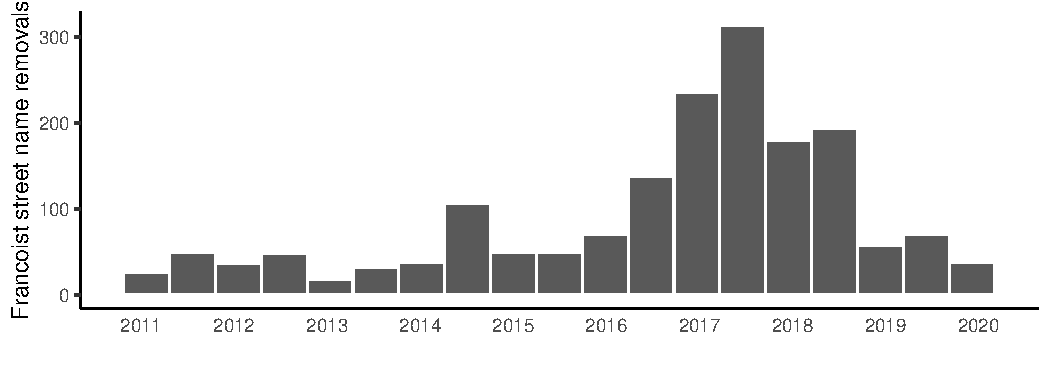
\includegraphics[width = 0.8\textwidth]{img/changes_over_time}

  \caption{Number of Francoist street name removals over time}\label{fig:changes_time}

\end{figure*}

\begin{figure*}[htb!]
\centering

  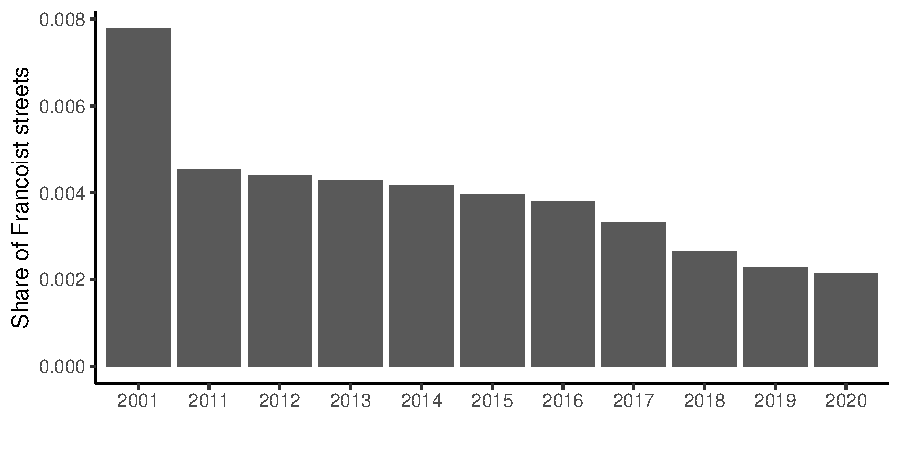
\includegraphics[width = 0.7\textwidth]{img/fs_year}

  \caption{Percentage of streets with Francoist street names over time}\label{fig:fs_year}

\end{figure*}

We use a binary indicator of Francoist street name removal in all the main models.
In the appendix, we show that the results do not change if we use a continuous measure (logged number of changes) instead.

\subsection*{Vox electoral support}

We exploit support for Vox as our main dependent variable, using it as a proxy for an authoritarian backlash in political preferences.
We obtained the data from the Spanish Ministry of Interior.\footnote{Results are available at \href{http://www.infoelectoral.mir.es/}{http://www.infoelectoral.mir.es/} (accessed 03/12/2020).}
We calculate the share of valid votes for Vox in each municipalities, as well as the change in support from April 2019 and November 2019 elections for some of the cross-sectional models.

In the difference-in-differences analyses, we also use as dependent variables the electoral share for the two mainstream parties, the right-wing Popular Party (\textit{Partido Popular}, PP) and the Spanish Socialist Workers' Party (\textit{Partido Socialista Obrero Español}, PSOE), in order to capture the local shift in political preferences.
Specifically, given that we are interested in a potential authoritarian backlash among conservative individuals, we want to explore whether the removal of Francoist street names is related to a general shift to the right or an increase in political polarization.

\subsection*{Control variables}

We include a series of control variables that can be related to electoral support for Vox.
In the cross-sectional analyses on electoral results in 2019, we include turnout, the (logged) population in the 2011 census, and the local unemployment rate in January 2011.
In the difference-in-differences analyses, we include population, unemployment rate in January 2016, the (logged) number of Francoist streets in June 2016, and whether a leftist mayor was elected in the 2015 local elections.
In every case, we also include fixed effects at the region level (Autonomous Communities).

\subsection*{Models}

We build two sets of models.
The cross-sectional analyses use a linear regression on the vote share of Vox in both 2019 elections (April and November), as well as the change between them, using as the main independent variable a binary indicator of street name removal between June 2001 and January 2019.
We use both a full sample of Spanish municipalities and a restricted sample of those municipalities that had at least one street with Francoist name in June 2001.

In the difference-in-differences analyses, we use linear regression on electoral support for Vox, PP, and PSOE in June 2016 and April 2019 elections, using as our main independent variable an indicator of street name removal between June 2016 and January 2019.
In these models, we only compare municipalities that had at least one street with Francoist name at the beginning of the period.

We include a series of additional models in the appendix to test the robustness of the results.
In particular, we include pre-treatment placebos to test the parallel trends assumption, include two different specifications of the name removal variable (in continuous form, and extending changes to the first half of 2019), and restrict the sample to municipalities where Vox got more than 0 votes in June 2016.

\section*{Results}

Table~\ref{tab:main_cs} shows the results of the cross-sectional analyses using the whole sample.
The first two columns show that the removal of Francoist street names between June 2001 and December 2018 is correlated with a higher electoral support for Vox in both April and November 2019 elections.
The third column, however, shows that there is no correlation with the change in support between these two elections.

\begin{table}[!htbp] \centering
  \caption{Francoist street name removal and electoral support for Vox}
  \label{tab:main_cs}
\small
% \begin{tabular}{@{\extracolsep{-20pt}}lD{.}{.}{-3} D{.}{.}{-3} D{.}{.}{-3} }
\begin{tabular}{lccc}
\\[-1.8ex]\hline
\hline \\[-1.8ex]
\\[-1.8ex] & \multicolumn{1}{c}{\footnotesize Apr 2019} & \multicolumn{1}{c}{\footnotesize Nov 2019} & \multicolumn{1}{c}{\footnotesize Change} \\
\\[-1.8ex] & \multicolumn{1}{c}{(1)} & \multicolumn{1}{c}{(2)} & \multicolumn{1}{c}{(3)}\\
\\[-1.8ex]\hline
\\[-1.8ex]
 (Intercept) & 0.078^{***} & 0.147^{***} & 2.195^{***} \\
  & (0.009) & (0.010) & (0.119) \\
  Francoist street name removal & 0.010^{***} & 0.013^{***} & -0.015 \\
  & (0.002) & (0.002) & (0.020) \\
  Unemployment 2019 & 0.084^{***} & 0.195^{***} & 0.518 \\
  & (0.025) & (0.031) & (0.337) \\
  Turnout April 2019 & 0.005 &  & -0.623^{***} \\
  & (0.010) &  & (0.133) \\
  Turnout Nov 2019 &  & -0.038^{***} &  \\
  &  & (0.011) &  \\
  Log. Population & 0.003^{***} & 0.006^{***} & -0.009^{+} \\
  & (0.000) & (0.000) & (0.005) \\
 \hline \\[-1.8ex]
CCAA Fixed Effects & \multicolumn{1}{c}{Yes} & \multicolumn{1}{c}{Yes} & \multicolumn{1}{c}{Yes} \\
Observations & \multicolumn{1}{c}{7,819} & \multicolumn{1}{c}{7,820} & \multicolumn{1}{c}{7,552} \\
R$^{2}$ & \multicolumn{1}{c}{0.442} & \multicolumn{1}{c}{0.500} & \multicolumn{1}{c}{0.078} \\
Adjusted R$^{2}$ & \multicolumn{1}{c}{0.441} & \multicolumn{1}{c}{0.498} & \multicolumn{1}{c}{0.075} \\
\hline
\hline \\[-1.8ex]
\multicolumn{4}{c}{\parbox[t]{0.7\textwidth}{\textit{Note:} $+ p<0.1; * p<0.05; ** p<0.01; *** p<0.001$. The main independent variable refers to the removal of Francoist street names between June 2001 and December 2018.}} \\
\end{tabular}
\end{table}

An obvious concern for these results is that left-leaning municipalities had already removed Francoist street names before 2001.
To account for this, table~\ref{tab:main_cs} repeats these analyses using a limited sample of those municipalities that still had streets with Francoist names in June 2001.
The results mirror the previous ones, although effect sizes are relatively smaller.
In the appendix, we show equivalent analyses but only including street name removals after the 2007 Law of Historical Memory was passed, namely, between 2011 and 2018.
Results do not change significantly.

% Table created by stargazer v.5.2.2 by Marek Hlavac, Harvard University. E-mail: hlavac at fas.harvard.edu
% Date and time: Tue, Nov 24, 2020 - 19:01:12
% Requires LaTeX packages: dcolumn
\begin{table}[!htbp] \centering
  \caption{Francoist street name removal and electoral support for Vox}
  \label{tab:cs_limited}
\small
% \begin{tabular}{@{\extracolsep{-20pt}}lD{.}{.}{-3} D{.}{.}{-3} D{.}{.}{-3} }
\begin{tabular}{lccc}
\\[-1.8ex]\hline
\hline \\[-1.8ex]
\\[-1.8ex] & \multicolumn{1}{c}{\footnotesize Apr 2019} & \multicolumn{1}{c}{\footnotesize Nov 2019} & \multicolumn{1}{c}{\footnotesize Change} \\
\\[-1.8ex] & \multicolumn{1}{c}{(1)} & \multicolumn{1}{c}{(2)} & \multicolumn{1}{c}{(3)}\\
\hline \\[-1.8ex]
 (Intercept) & 0.119^{***} & 0.211^{***} & 2.362^{***} \\
  & (0.018) & (0.020) & (0.156) \\
  Francoist street name removal & 0.005^{*} & 0.008^{**} & 0.003 \\
  & (0.002) & (0.003) & (0.019) \\
  Unemployment 2019 & 0.043 & 0.141^{*} & 0.450 \\
  & (0.047) & (0.058) & (0.404) \\
  Turnout April 2019 & -0.020 &  & -0.799^{***} \\
  & (0.020) &  & (0.178) \\
  Turnout Nov 2019 &  & -0.086^{***} &  \\
  &  & (0.023) &  \\
  Log. Population & 0.002^{*} & 0.003^{***} & -0.018^{**} \\
  & (0.001) & (0.001) & (0.006) \\
 \hline \\[-1.8ex]
CCAA Fixed Effects & \multicolumn{1}{c}{Yes} & \multicolumn{1}{c}{Yes} & \multicolumn{1}{c}{Yes} \\
Observations & \multicolumn{1}{c}{2,164} & \multicolumn{1}{c}{2,165} & \multicolumn{1}{c}{2,153} \\
R$^{2}$ & \multicolumn{1}{c}{0.292} & \multicolumn{1}{c}{0.318} & \multicolumn{1}{c}{0.134} \\
Adjusted R$^{2}$ & \multicolumn{1}{c}{0.284} & \multicolumn{1}{c}{0.311} & \multicolumn{1}{c}{0.125} \\
\hline
\hline \\[-1.8ex]
\multicolumn{4}{c}{\parbox[t]{0.7\textwidth}{\textit{Note:} $+ p<0.1; * p<0.05; ** p<0.01; *** p<0.001$. The main independent variable refers to the removal of Francoist street names between June 2001 and December 2018. Only municipalities that had Francoist street names in June 2001 were included.}} \\
\end{tabular}
\end{table}

Results point to a relationship between the removal of Francoist names and increased support for the new far-right party Vox.
The absence of a correlation between Francoist name removals and the change in support for Vox throughout 2019 suggests that any local effect due to a backlash over the politics of memory took place prior to April 2019.
This result is relevant because the historical memory of the conflict was particularly present during the electoral campaign prior to the November 2019 elections, particularly because of the exhumation of Franco's remains that same month.
Thus, we could have expected that this campaign mobilized the voters who were discontent with the 2007 Law of Historical Memory.
But, if anything, the results suggest that the effect of this cleavage on voting preferences was already present before.

It is difficult to talk about any causal effect with these cross-sectional analyses.
To get closer to a causal identification, we develop a difference-in-differences setup where we analyze the increase in electoral support for Vox between 2016 and 2019 elections, the period during which the party grew from being politically irrelevant (with marginal political influence) to becoming a relevant party at the national level.
We also analyze the change in support for the main two parties, PSOE and PP, to check whether any change is related to an increase in polarization or to a general shift to rightist positions.

Table~\ref{tab:main_DiD} shows the results of the DiD analyses.
Each of the three columns shows the results for the same model using electoral support for the three different parties: Vox, PP, and PSOE.
In order to see the results more clearly, figure~\ref{fig:main_DiD} shows the simulated DiD estimate of the Francoist street name removal.
In other words, the effect of the street name removal on the change in electoral support for these parties between 2016 and 2019.

\begin{table}[!htbp] \centering
  \caption{Francoist street name removal and increase in electoral support for parties}
  \label{tab:main_DiD}

  \small
  \begin{tabular}{lccc}
  \\[-1.8ex]\hline
  \hline \\[-1.8ex]
  \\[-1.8ex] & \multicolumn{1}{c}{VOX} & \multicolumn{1}{c}{PP} & \multicolumn{1}{c}{PSOE} \\
  \\[-1.8ex] & \multicolumn{1}{c}{(1)} & \multicolumn{1}{c}{(2)} & \multicolumn{1}{c}{(3)}\\
  \\[-1.8ex]\hline
  \\[-1.8ex]
   (Intercept) & -1.470^{**} & 56.375^{***} & 34.870^{***} \\
    & (0.451) & (0.922) & (0.876) \\
    Francoist street name removal & -0.132 & 1.158^{*} & -0.159 \\
    & (0.262) & (0.476) & (0.453) \\
    Election April 2019 & 12.319^{***} & -17.406^{***} & 4.629^{***} \\
    & (0.167) & (0.338) & (0.320) \\
    Francoist removal $\times$ April 2019 & 0.724^{*} & -1.405^{*} & -0.434 \\
    & (0.352) & (0.639) & (0.607) \\
   \hline \\[-1.8ex]
  Controls & \multicolumn{1}{c}{Yes} & \multicolumn{1}{c}{Yes} & \multicolumn{1}{c}{Yes} \\
  CCAA Fixed Effects & \multicolumn{1}{c}{Yes} & \multicolumn{1}{c}{Yes} & \multicolumn{1}{c}{Yes} \\
  $n$ & \multicolumn{1}{c}{2,310} & \multicolumn{1}{c}{3,223} & \multicolumn{1}{c}{3,242} \\
  R$^{2}$ & \multicolumn{1}{c}{0.768} & \multicolumn{1}{c}{0.720} & \multicolumn{1}{c}{0.482} \\
  Adjusted R$^{2}$ & \multicolumn{1}{c}{0.766} & \multicolumn{1}{c}{0.717} & \multicolumn{1}{c}{0.478} \\
  \hline
  \hline \\[-1.8ex]
  \multicolumn{4}{c}{\parbox[t]{0.75\textwidth}{\textit{Note:} + $p<0.1$; * $p<0.05$; ** $p<0.01$; *** $p<0.001$. Controls include a dummy for a leftist major elected in 2015 local elections, logged population in 2011, logged number of Francoist streets in $t_{0}$, and the unemployment rate in January 2016. Only municipalities that had at least one street with a Francoist name in $t_{0}$ (June 2016) were included in the sample.}} \\
  \end{tabular}
\end{table}

\begin{figure*}[htb!]
\centering

  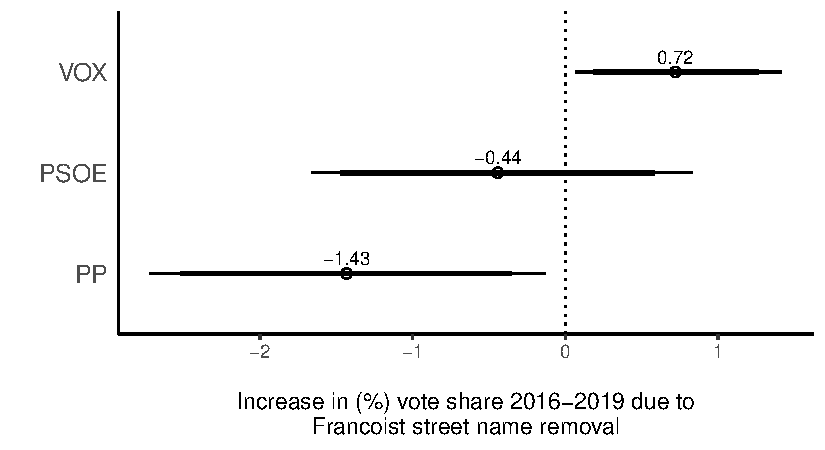
\includegraphics[width = 0.6\textwidth]{../output/DiD_estimates}

  \caption{difference-in-differences estimates of Francoist street name removal on vote change, obtained from 1000 simulations. Points show the mean estimate, bars indicate 90\% and 95\% CIs.}\label{fig:main_DiD}

\end{figure*}

Results support the idea that the name removal caused an authoritarian backlash.
On the one hand, in municipalities where Francoist street names were removed, Vox increased its support 0.7 points more.
Considering that the nation-wide electoral share of Vox was 10.3\%, this effect is significant.
In particular, it means that the change in electoral support was around 6\% higher in these municipalities.
On the other hand, the removal of Francoist street names is related to an even higher decrease in electoral support for PP, of almost 1.5 points, but it did not have any significant effect on electoral support for PSOE.
This last result suggest that this policy might have increased political polarization in Spain, given that the change in political preferences seems to have taken place within conservative individuals.
There is no evidence of a general shift to the right.

These results could be confounded if the removal of Francoist street names was explained by the same factors that also explain a shift to far-right preferences.
One possibility is that these street name changes, which took place relatively late, took place in more conservative areas where Spanish nationalism was stronger.
However, there are reasons to think that this concern should not invalidate the results.
First, the fact that we are only comparing municipalities that still had Francoist street names in mid-2016 means that conservative areas are already overrepresented in the sample.
The specific political factors that contributed to the change in street names---a leftist mayor elected in 2015 or the outcome of legal battles fought by local memory associations, for example---should be independent from the increase in support for Vox.
Second, if the concern above were true, we should see different trends before 2016 between municipalities that later had a change and those that did not.
However, in the appendix we include models with pre-treatment placebos for Vox and PP, which show that the parallel trends assumption holds.

Moreover, we show in the appendix additional analyses that test the robustness of the results to different specifications.
In addition to the inclusion of pre-treatment data, we also include the dependent variable in continuous form (logged number of street name removals), restrict the sample to municipalities where Vox had more than 0 votes in 2016, and change the independent variable so it also includes changes that were registered in the first half of 2019, to account for possible delays in the official data.
Results do not change in any of these specifications.

\section*{Conclusion}

In this article, we have explored the political effect of the removal of Francoist street names in Spain.
Our results suggest that this type of transitional justice policy might generate a backlash.
In particular, using local-level data, we find a short-term positive effect of these these changes on the increase in support for the far-right party Vox, a party that has recently gained steam with a discourse grounded in an authoritarian and exclusive version of Spanish nationalism.

The results from our analyses echo recent debates about TJ policies and memories of past conflicts in other countries. For example, the debate in the United States over the Confederate symbols shows that this type of policies can generate political instability and even violence. We show there is room for concern: revisiting the past and trying to redress the victims' grievances might cause a backlash among those ideologically closer to the perpetrator, leading to increased political polarization.

Far from arguing against these types of policies, we think it is important to be aware of these potentially undesired effects when designing transitional justice policies. Specifically, two aspects merit further attention.
First, here we show evidence of a short-term backlash effect. Yet, we do not know what happens in the longer term, particularly whether these policies produce a reconciliation effect down the road. Second, even if the removal of public symbols might cause backlash, the findings of this article do not necessarily apply to other transitional justice policies. For instance, recent research shows that transitional justice museums might have a positive effect on reconciliation \citep{Balcells:2020aa}.

All in all, this article focuses on a relatively unexplored question. Exploiting recent political events in Spain, we offer empirical evidence suggesting that symbolic transitional justice policies can generate backlash. %Events such as the violence that unfolded in  Charlottesville in 2017 are thus not isolated events; they are part of a broader pattern of backlash when particular symbols from the past are removed from public spaces.

\clearpage
\bibliographystyle{rap}
% \bibliography{ref}
\bibliography{$HOME/Documents/REF}$

\end{document}
